  \newcolumntype{C}{ >{\centering\arraybackslash} m{8cm} }
  \newcolumntype{D}{ >{\centering\arraybackslash} m{6cm} }
  \begin{tabular}{DC}
    CNF\ formula &{\scriptsize
          \begin{tabular}{c}
          	$ \{ x_{1}, x_{2}, x_{3} \}$,
          	$ \{ x_{4}, x_{5}, x_{6} \}$,
          	$ \{ x_{1}, x_{4} \}$ \\
          	$ \{ x_{2}, x_{5} \}$,
          	$ \{ x_{3}, x_{6} \}$ ,
          	$ \{ \neg x_{1}, \neg x_{2} \}$ \\
          	$ \{ \neg x_{1}, \neg x_{3} \}$,
          	$ \{ \neg x_{2}, \neg x_{3} \}$,
          	$ \{ \neg x_{4}, \neg x_{5} \}$\\
          	$ \{ \neg x_{4}, \neg x_{6} \}$,
          	$ \{ \neg x_{5}, \neg x_{6} \}$            
          \end{tabular}}\\
      & \\
    $\Downarrow$ & $\Downarrow$  \\
          & \\
    colored graph & 		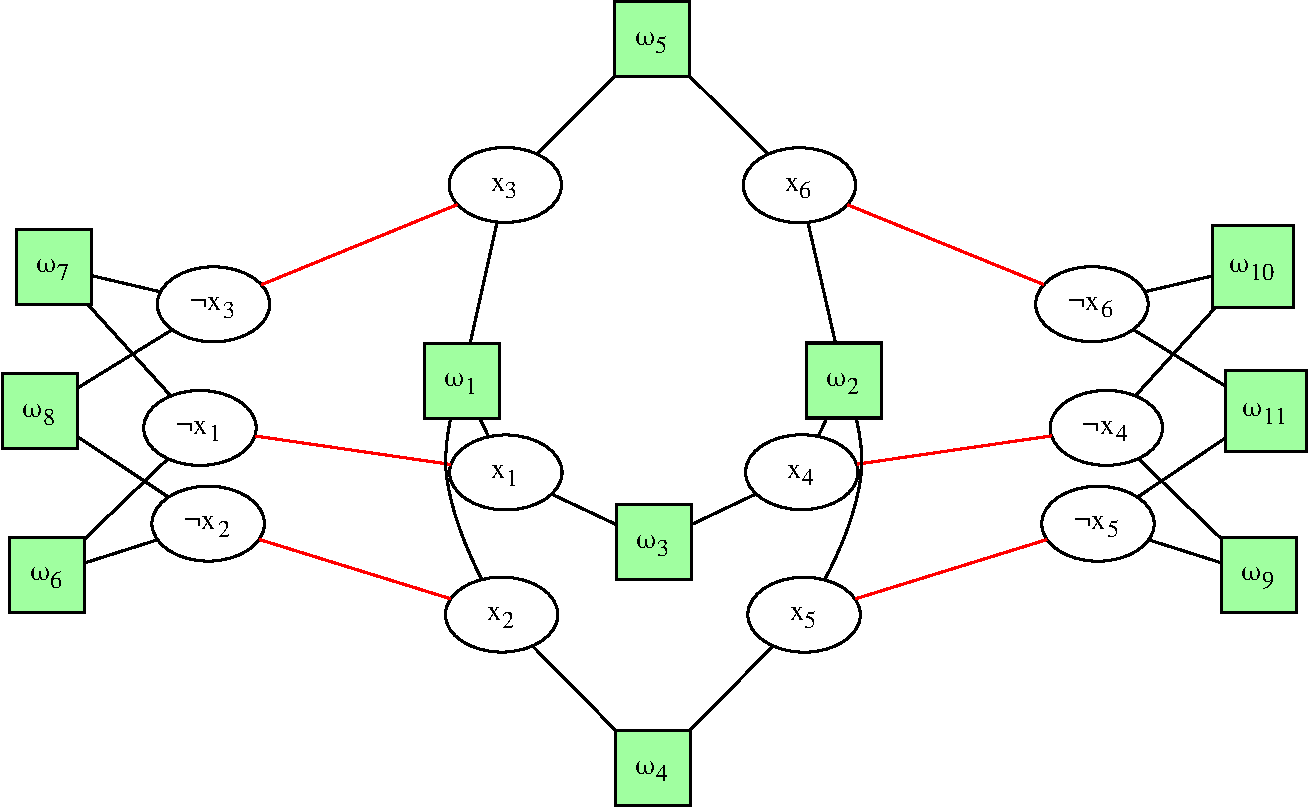
\includegraphics[width=2.5in]{cnfs/graph_cnf_no_opt-crop}\\

    $\|$ & $\|$  \\
        & \\
    graph automorphism &
                         \small{(\texttt{bliss} \footnote{http://www.tcs.hut.fi/Software/bliss/} or
                         \texttt{saucy} \footnote{http://vlsicad.eecs.umich.edu/BK/SAUCY/})}
    \\
  
        & \\
    $\Downarrow$ & $\Downarrow$  \\
      & \\
    set of symmetries & \begin{minipage}[l]{\textheight}
    	\footnotesize
    	$g_1 = (x_2 \enskip x_3)(x_5 \enskip x_6)(\neg x_2 \enskip \neg x_3)(\neg x_5 \enskip \neg x_6)$\\
    	$g_2 = (x_1 \enskip x_2)(x_4 \enskip x_5)(\neg x_1 \enskip \neg x_2)(\neg x_4 \enskip \neg x_5)$\\
    	$g_3 = (x_1 \enskip x_4)(x_2 \enskip x_5)(x_3 \enskip x_6)(\neg x_1 \enskip \neg x_4)(\neg x_2 \enskip \neg x_5)(\neg x_3 \enskip \neg x_6)$
    \end{minipage}  \\
  \end{tabular}